\chapter{Literature Review}
\label{chap:review}

This chapter covers the first task of this thesis project, which is the review of the literature on neuroevolution algorithms and benchmarks.
The first goal of this review is to identify the state of the art algorithms and benchmarks which were proposed in the neuroevolution theoretical and applied literature, with a particular
focus on the recent theory literature from 2023 and 2024. Following this, a selection of algorithms and benchmarks from the ones which were identified is made.
This selection consists in the algorithms and benchmarks which are presented in detail in this section and which are implemented in the framework.

\section{Methodology}

Given the large amount of literature on this well-established field, the review was conducted in a systematic manner, following the guidelines of \cite{snowballing,systematic_review}.
Indeed, using a rigid methodology is cruucial in order to ensure that the review is impartial and precise.

\subsection{Research Questions}

The research goals are summarized in the following research questions:

\begin{itemize}
    \item \textbf{RQ1:} What are the state of the art neuroevolution algorithms?
    \item \textbf{RQ2:} What are the different kinds of neuroevolution algorithms?
    \item \textbf{RQ3:} Which benchmarks are used to evaluate neuroevolution algorithms?
    \item \textbf{RQ4:} What are the key characteristics of these different benchmarks?
\end{itemize}

\textbf{RQ1} and \textbf{RQ3} are concerned with the identification of the state of the art algorithms and benchmarks, while \textbf{RQ2} and \textbf{RQ4} are concerned
with the selection process.

\subsection{Search Strategy}

The search for papers was performed using Google Scholar and the DTU Findit database, which should provide an accurate representation fo the research that has been
conducted on the topic. The keywords used for designing the search queries are:

\begin{quote}
    "Neuroevolution", "Neural Networks", "Evolution Algorithm", "Evaluation"
\end{quote}

\subsection{Study Selection}

Following the queries on the databases, the results are then filtered based on the title, abstract and full-text reading (in this order). An iteration of forward
and backward snowballing were then conducted to include other studies which were missed in the initial search.

The following inclusion criteria were applied to the abstracts:

\begin{itemize}
    \item \textbf{IC1:} The paper is published after 2002.
    \item \textbf{IC2:} It is clear that the work is proposing a new noeuroevolution algorithm or performing an evaluation of existing algorithms.
    \item \textbf{IC3:} The considered algorithm(s) rely solely on evolutionary algorithms.
    \item \textbf{IC4:} The considered algorithm(s) aim at the evolution of weights, and possibly topologies, of artificial neural networks.
\end{itemize}

And the following exclusion criteria were used:

\begin{itemize}
    \item \textbf{EC1:} The paper is not available in English.
    \item \textbf{EC2:} The full=text of the paper is not accessible
    \item \textbf{EC3:} The study is a duplicate of a previously included study.
\end{itemize}

The cut-off date of 2002 is motivated by the release year of the \cite{neat} paper, proposing the NEAT algorithm, which is the most studied neuroevolution algorithm and which
is still the subject of many studies today.

\section{Neuroevolution algorithms}

A variety of neuroevolution algorithms have been proposed in the literature.
These algorithms can be classified into different categories based on their main characteristics.
The following three main distinctions, which were mentioned in \Cref{chap:background}, have been identified during the review:

\begin{itemize}
    \item \textbf{Conventional neuroevolution algorithms vs. TWEANNs} Conventional neuroevolution algorithms are those which only evolve the connection weights,
        considering a fixed topology, while TWEANNs (Topology and Weight Evolving Artificial Neural Networks) \cite{neat} are those which also evolve the topology of the
        neural network.
    \item \textbf{The category of the evolutionary algorithm} such as genetic algorithms \cite{genetic_alg,genetic_alg_review}, evolutionary strategies \cite{es_intro},
        genetic programming \cite{cartesian_gp}.
    \item \textbf{The encoding strategy} This refers to the way the neural network is encoded as a genotype, \cite{neuroevolution_learning,neuroevolution_trends,neuroevolution_survey}.
        The most common encoding strategies are direct encoding, indirect encoding and generative encoding.
\end{itemize}

\Cref{tab:neuroevolution_algorithms} presents a classification of the neuroevolution algorithms which were identified during the review.
Various algorithms were identified for each of the categorie, such as different evolution strategies, an approach relying on Cartesian genetic programming, an anglrotihm not evolving the
weights, or an algorithm proposing an entirely new evolutionary method.

\begin{table}[]
\caption{Neuroevolution algorithms classification}
\label{tab:neuroevolution_algorithms}
\centering
\begin{tabular}{|c|c|c|c|}
\hline
\textbf{Algorithm}  & \textbf{Evolves topologies} & \textbf{EA category}                                                             & \textbf{Encoding strategy}                                          \\ \hline
\textbf{NEAT} \cite{neat}     & Yes                         & Genetic Algorithm                                                                & Direct                                                    \\ \hline
\textbf{CMA-ES} \cite{cmaes}  & N/A                         & Evolution strategies                                                             & N/A                                                       \\ \hline
\textbf{(1 + 1) NA} \cite{na} & No                          & Genetic Algoerithm                                                               & Direct                                                    \\ \hline
\textbf{BNA} \cite{bna}       & No                          & Genetic Algorithm                                                                & Direct                                                    \\ \hline
HyperNEAT \cite{hyperneat}    & Yes                         & Genetic Algorithm                                                                & Indirect                                                  \\ \hline
CGPANN \cite{cgpann}          & Yes                         & Genetic Programming                                                              & Direct                                                    \\ \hline
CoSyNE \cite{cosyne}          & No                          & Genetic Algorithm                                                                & Direct                                                    \\ \hline
AGE \cite{age}                & Yes                         & Genetic Algorithm                                                                & Indirect                                                  \\ \hline
WANNs \cite{wanns}            & Yes (not the weights)       & Genetic Algorithm                                                                & Direct                                                    \\ \hline
EANT2 \cite{eant2}            & Yes                         & \begin{tabular}[c]{@{}c@{}}Genetic Algorithm\\ Evolution Strategies\end{tabular} & \begin{tabular}[c]{@{}c@{}}Direct\\ Indirect\end{tabular} \\ \hline
xNES \cite{xnes}              & N/A                         & Evolution Strategies                                                             & N/A                                                       \\ \hline
OpenAI ES \cite{openai_es}    & N/A                         & Evolution Strategies                                                             & N/A                                                       \\ \hline
SUNA \cite{suna}              & Yes                         & Specific evolutionary method                                                     & Direct                                                    \\ \hline
\end{tabular}
\end{table}

\subsection{Algorithms selection}

The following algorithms were selected for the implementation in the framework:

\begin{itemize}
    \item The (1 + 1) NA algorithm and its variants
    \item The Bias-Invariant (1+1) NA (BNA) algorithm
    \item The CMA-ES Evolutionary Strategy
    \item The NEAT algorithm
\end{itemize}

Given the duration of the project, the choice was made to limit the number of algorithms to four, in order to allow for an in-depth implementation and evaluation of
each of them, thus various criteria were used for the selection of the algorithm, to allow for a good coverage of the different categories of algorithms and
interesting comparisons between them.

The (1 + 1) NA and bias-invariant (1+1) NA algorithms were selected as the two theory paper proposals this thesis is particularly interested in.
The CMA-ES algorithm, which is the representative of the evolutionary strategies category was selected because of its popularity in the modern neuroevolution literature
and applications, and because of its status as a state-of-the-art algorithm for continuous optimization problems.
Finally, the NEAT algorithm, the representative of the TWEANN category, was selected because of its status as the most well-known neuroevolution algorithm, making
it a subject of the vast majority of the comparison studies in the literature, and as a baseline for the evaluation of new algorithms.

The following sections present the selected algorithms in detail.

\subsection{(1 + 1) NA}

The (1 + 1) NA algorithm and its variants were introduced in \cite{na}.
In this work, the authors consider a simple neuroevolution setting where these algorithms are used to optimize the weights and activation function of
a simple artificial neural network.

\subsubsection{The artificial neural network topology}

Artificial neurons with $D$ inputs and a binary threshold activation function are considered.
These neurons have $D + 1$ parameters, the input weights $w_1, \ldots, w_D$ and the threshold $t$.
Let $x = (x_1, \ldots, x_D) \in \mathds{R}^D$ be the input of the neuron. The neuron outputs $1$ if $\sum_{i=1}^D w_i x_i \geq t$ and $0$
otherwise.
This can be interpreted geometrically as the neuron outputting $1$ if the input vector $x$ is above or on the hyperplane with normal vector
$w = (w_1, \ldots, w_D)$ and bias $t$.
j
Furthermore, an alternative representation of the decision hyperplane can be used by considering spherical coordinates.
The decision hyperplane is described by its normal vector, which is characterized by by $D - 1$ angles, and by the bias, which corresponds to the distance from the origin
measured in the opposite direction of that of the normal vector.
For example, for $D = 2$, the normal vector can be represented by its cartesian coordinates $(x_1, x_2)$ or by its polar coordinates
$(r, \theta)$, where $r$ is the distance from the origin and $\theta$ is the angle with the $x_1$ axis. Similarly, for $D = 3$, the normal vector can
be represented by its cartesian coordinates $(x_1, x_2, x_3)$ or by its spherical coordinates $(r, \theta, \phi)$, where $r$ is the distance from the
origin, $\theta$ is the angle with the $x_1$ axis and $\phi$ is the angle with the $x_3$ axis.
It is easy to convert between these two representations \cite{spherical}. In addition, the spherical representation uses one less parameter than the cartesian
representation, and hence, allows for the reduction of the number of inputs to the neurons to $D$, as opposed to $D + 1$ when using the cartesian representation,
where $D$ parameters are used for the normal vector and $1$ for the bias.

% TODO coordinates figure

The ANNs which are considered in the study contain three layers: the input layer, a hidden layer with $N > 1$ neurons and an output layer with a single neuron.
Each of the hidden neurons are connected to the $D$ inputs and output a binary value. The output neuron is connected to the $N$ hidden neurons and
computes the Boolean OR function of their outputs.
This architecture is motivated by the problems which are considered in the study \cite{na}.
Geometrically, these ANNs output the union of a number of $N$-dimensional hyperplanes.
\Cref{fig:oneplusonena_ann} shows the structure of the ANNs evolved by the (1 + 1) NA algorithm.

\begin{figure}
    \begin{center}
        \begin{tikzpicture}[shorten >=1pt,->,draw=black!50, node distance=\layersep]
            \tikzstyle{every pin edge}=[<-,shorten <=1pt]
            \tikzstyle{neuron}=[circle,fill=black!25,minimum size=17pt,inner sep=0pt]
            \tikzstyle{input neuron}=[neuron, fill=green!50];
            \tikzstyle{output neuron}=[neuron, fill=red!50];
            \tikzstyle{hidden neuron}=[neuron, fill=blue!50];
            \tikzstyle{annot} = [text width=4em, text centered]

            % Input layer nodes
            \foreach \name / \y in {1,2}
                \node[input neuron] (I-\name) at (0,-\y) {};

            \node at (0,-3) {$\vdots$};

            \node[input neuron] (I-4) at (0,-4) {};

            \foreach \name / \y in {1,...,5}
                \path[yshift=0.5cm]
                    node[hidden neuron] (H-\name) at (\layersep,-\y cm) {};

            \node[output neuron, right of=H-3] (O) {OR};

            \foreach \source in {1,2,4}
                \foreach \dest in {1,...,5}
                    \path (I-\source) edge (H-\dest);

            \foreach \source in {1,...,5}
                \path (H-\source) edge (O);

            \node[annot,above of=H-1, node distance=1cm] (hl) {Hidden layer (N neurons)};
            \node[annot,left of=hl] {Input layer (D neurons)};
            \node[annot,right of=hl] {Output layer (1 neuron)};
        \end{tikzpicture}
        \caption{Structure of the ANNs evolved by the (1 + 1) NA algorithm}
        \label{fig:oneplusonena_ann}
    \end{center}
\end{figure}

\subsubsection{The (1 + 1) NA algorithm}

Let's consider an ANN with $N$ neurons in the hidden layer and $D$ inputs, with parameters
$(\phi_{1,1}, \dots, \phi_{1,D-1}, b_1, \dots, \phi_{N,1}, \dots, \phi_{N,D-1}, b_N$.
In \cite{na}, the search space $[0 , \dots, n]^{N D}$ is considered, where $r$ is the resolution of the continuous $[0, 1]$ domain.
This discretiisation allows for the values $\{0, 1/r, 2/r, \dots, 1\}$. Setting the parameters of ANNs is tipically a continous optimization problem,
but rigurous runtime analysis is much less developed for continous optimization than for discrete optimization, which motivates this choice.
Let $f : \{0 , \dots, r\}^{N D} \to [0, 1]$ be the fitness function which measures the performance of the ANN and is to be maximized.

The (1 + 1) NA algorithm is given in \Cref{alg:na}.
It maintains a single individual and mutates all angles and biases independently, based on a global search operator using the harmonic distribution
$\text{Harm}(r)$ on $\{1, \dots, r\}$: For $l \sim \text{Harm}(r)$,

\[
    Prob(l = i) = \frac{1}{H_r} \text{ for } i = 1, \dots, r, \text{ where } H_r = \sum_{i=1}^r \frac{1}{i}.
\]

\begin{algorithm}
\caption{(1 + 1) NA}
\label{alg:na}
\begin{algorithmic}
    \State $t \gets 0$
    \State Select $x_0$ uniformly at random from $\{0, \ldots, r\}^{DN}$.
    \While{termination criterion not met}
        \State Let $y = (\varphi_{1,1}, \ldots, \varphi_{1,D-1}, b_1, \ldots, \varphi_{N,1}, \ldots, \varphi_{N,N-1}, b_N) \gets x_t;$
        \ForAll{$i \in \{1, \ldots, N\}$}
            \State Mutate $\varphi_{i,1} \dots, \varphi_{i,D}$ and $b_i$ with probability $\frac{1}{DN}$, independently of each other and other indices;
            \State Mutation chooses $\sigma \in \{-1, 1\}$ uniformly at random and $l \sym \text{Harm}(r)$ and adds $\sigma l$ to the selected component, the
            result is then taken modulo $r$ for angles and modulo $r + 1$ for biases.
            \For {$i \in \{1, \ldots, N\}$}
                \State Set bias $2b_i / r - 1$ for neuron $i$.
                \For {$j \in \{1, \ldots, D\}$}
                    \State Set the $j$-th polar angle to $2\pi \varphi_{i,j} / r$ for neuron $i$.
                \EndFor
            \EndFor
            \State Evaluate $f(y)$
            \If{$f(y) \geq f(x_t)$}
                \State $x_{t+1} \gets y$
            \Else
                \State $x_{t+1} \gets x_t$
            \EndIf
        \EndFor
        \State $t \gets t + 1$
    \EndWhile
\end{algorithmic}
\end{algorithm}

\subsubsection{The evaluation in practice}

The ANNs which are evolved using the (1 + 1) NA algorithm output the union of $N$-dimensional hyperplanes. To check whether or not the input is above the
hyperplane described by one of the neurons, the normal vector $\overrightarrow{n}$ to the hyperplane is computed using the angles and a norm of $1$.
For an input vector $\overrightarrow{x}$, the dot product $(\overrightarrow{x} - \lvert b \rvert \overrightarrow{n}) \cdot \overrightarrow{n}$ is computed, where
$b$ is the bias of the neuron. If $b \geq 0$, the output of the neuron is $1$ if the dot product is positive and $0$ otherwise. If $b < 0$,
the output of the neuron is $1$ if the dot product is negative and $0$ otherwise.

\subsection{Bias-Invariant (1+1) NA (BNA)}

In \cite{bna}, the authors extend upon the analysis in \cite{na} by considering more realistic ANN settings, presenting the Bias-Invariant (1+1) NA (BNA) algorithm.
The considered ANNs uses Rectified-Linear-Unit (ReLU) activation functions, commonly used in real-world ANNs.
This allows for the construction of bended hyperplanes, resulting in solutions to the problems described in \cite{na} which are invariant to the bias.

\subsubsection{The artificial neural network topology}

The considered ANNs contain three layers, in which each of the neurons uses a ReLU activation function i.e they output $\max(0, \sum_{i=1}^k w_i x_i)$ for
$k$ inputs from the previous layer.
The weights between the first and second layer and between the second and third layer are fixed. The topology for $D = 2$ in shown in \Cref{fig:bna-ann}.
The use of ReLU activation functions results in piecewise linear output. Hence, these networks compute a V-shaped area of positive classification. Such topologies are considered
as a single neuron, refered to as a \textbf{V-neuron}, and which can be part of a standard ANN topology. For example V-neurons can be used in the hidden layer of the (1 + 1) NA
ANNs \cite{na} to compute the union of V-shaped areas of positive classification.

Therefore, these V-neurons can be described by $D + 1$ parameters:

\begin{itemize}
    \item The bias $b$
    \item The $D - 1$ angles $\varphi_1, \ldots, \varphi_{D-1}$.
    \item The bend angle $\theta$.
\end{itemize}

The area of positive classification is a (multi-dimensional) cone, all points positively classified correspond to points forming an angle smaller than the bend
angle $\theta$ with the normal vector to the hyperplane given by the bias $b$ and the $D -1$ angles $\varphi_1, \ldots, \varphi_{D-1}$.
\Cref{fig:bna-cone} shows a visualization of the area of positive classification of a V-neuron for $D = 2$.

\begin{figure}
    \centering
    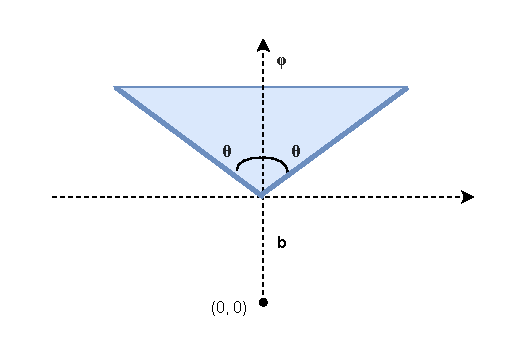
\includegraphics[width=0.7\textwidth]{Pictures/bna_cone}
    \caption{Visualization of the area of positive classification of a V-neuron for $D = 2$.}
    \label{fig:bna-cone}
\end{figure}

% TODO ANN figure

\subsubsection{The Bias-Invariant (1+1) NA algorithm}

The BNA algorithm is given in \Cref{alg:bna}.
It is mostly the same as the (1+1) NA algorithm, with the difference that the bend angles are also mutated.
In particular, it can be seen that when fixing the bend angles to $\pi / 2$, the BNA algorithm is equivalent to the (1+1) NA algorithm.

\begin{algorithm}
    \caption{Bias-Invariant (1 + 1) NA (BNA)}
\label{alg:bna}
\begin{algorithmic}
    \State $t \gets 0$
    \State Select $x_0$ uniformly at random from $\{0, \ldots, r\}^{DN}$.
    \While{termination criterion not met}
        \State Let $y = (\theta_1, \varphi_{1,1}, \ldots, \varphi_{1,D-1}, b_1, \ldots, \theta_N, \varphi_{N,1}, \ldots, \varphi_{N,N-1}, b_N) \gets x_t;$
        \ForAll{$i \in \{1, \ldots, N\}$}
            \State Mutate $\varphi_{i,1}, \dots, \varphi_{i,D}$, $\theta_i$ and $b_i$ with probability $\frac{1}{(D+1) N}$, independently of each other and other indices;
            \State Mutation chooses $\sigma \in \{-1, 1\}$ uniformly at random and $l \sym \text{Harm}(r)$ and adds $\sigma l$ to the selected component, the
            result is then taken modulo $r$ for angles and modulo $r + 1$ for biases.
            \For {$i \in \{1, \ldots, N\}$}
                \State Set bias $2b_i / r - 1$ for neuron $i$.
                \State Set bend angle $\pi \theta_i / r$ for neuron $i$.
                \For {$j \in \{1, \ldots, D\}$}
                    \State Set the $j$-th polar angle to $2\pi \varphi_{i,j} / r$ for neuron $i$.
                \EndFor
            \EndFor
            \State Evaluate $f(y)$
            \If{$f(y) \geq f(x_t)$}
                \State $x_{t+1} \gets y$
            \Else
                \State $x_{t+1} \gets x_t$
            \EndIf
        \EndFor
        \State $t \gets t + 1$
    \EndWhile
\end{algorithmic}
\end{algorithm}

\subsubsection{The evaluation}

V-neurons output whether or not the input is in the cone described by the neuron. The vector $\overrightarrow{\varphi}$ is computed using the angles $\varphi_1, \ldots, \varphi_{D-1}$
and a norm of $1$. Given an input vector $\overrightarrow{x}$, the dot product $(\overrightarrow{x} - \lvert b \rvert \overrightarrow{\varphi}) \cdot \overrightarrow{\varphi}$ is computed.
The angle $\alpha$ between the input vector and the normal vector can then be computed as
$\alpha = \cos^{-1}(\frac{(\overrightarrow{x} - \lvert b \rvert \overrightarrow{\varphi}) \cdot \overrightarrow{\varphi})}{\lVert \overrightarrow{x} - \lvert b \rvert \overrightarrow{\varphi} \rVert
\lVert \overrightarrow{\varphi} \rVert})$. If $b \geq 0$, the output of the neuron is $1$ if $\alpha \leq \theta$ and $0$ otherwise. If $b < 0$, the output of the neuron is
$1$ if $\pi - \alpha \leq \theta$ and $0$ otherwise.

\subsection{The CMA-ES Evolutionary Strategy}

CMA-ES \cite{cmaes}, short for \textit{Covariance Matrix Adaptation Evolution Strategy}, is a kind of evolution strategy (ES) \cite{es_intro}.
This kind of blax-box optimization algorithms aim at optimizing a function $f : \mathds{R}^n \to \mathds{R}$, for which the analytic form is not known,
but for which evaluations of the function are possible. As it ts the case for CMA-ESl these algorithms are typically stochastic and are used for the optimization of
non-linear or non-convex continuous variables optimization problems.

ES algorithms maintain a (parametrized) population of candidate solutions. These candidate solutions are sampled from a multivariate normal distribution. Parameters of the distribution
are updated at each generation based on the performance of the candidate solutions. As a matter of fact, a simple greedy ES algorithm could consist in updating the
mean of the distribution, and using a fixed standard deviation. The mean is updated to the best solution after the evaluation of the fitness of candidate
solutions. The next generation is then sampled around this mean. However, this kind of simple greedy algorithms is particularly prone to getting stuck at local optima because
of the lack of exploration.

In order to allow for more exploration, rather than exclusively relying on the single best solution, genetic algorithm maintain a proportion of the best solutions from
the current generation, and generate the next one trough recombinations and mutations. However, this approach is also prone to getting stuck at local optima, as in
practice, candidates solutions end up converging to a local optimum.

CMA-ES addresses these issues and allows for the adaption of the search space when needed, reducing it when the confidence in current solutions is high, for fine-tuning, or
increasing it when the confidence is low, in order to allow for more exploration. This is done by adapting the covariance matrix of the multivariate normal distribution,
which stores pairwise dependencies between the parameters for the sample distribution. This process is illustrated in \Cref{fig:cmaes_visualization}.
It makes CMA-ES a powerful and widely used optimization algorithm. The main drawback of this algorithm is its computational cost, induced by the use of the covariance matrix,
which makes it less suitable for high-dimensional problems.

CMA-ES can be used for the evolution of fixed-topology neural networks, by considering the weights of the connections as the parameters of the optimization problem,
and converting between a vector representation of the network, for the optimization input, and the standard graph representation, for the evaluation of individuals.

\begin{figure}
    \centering
    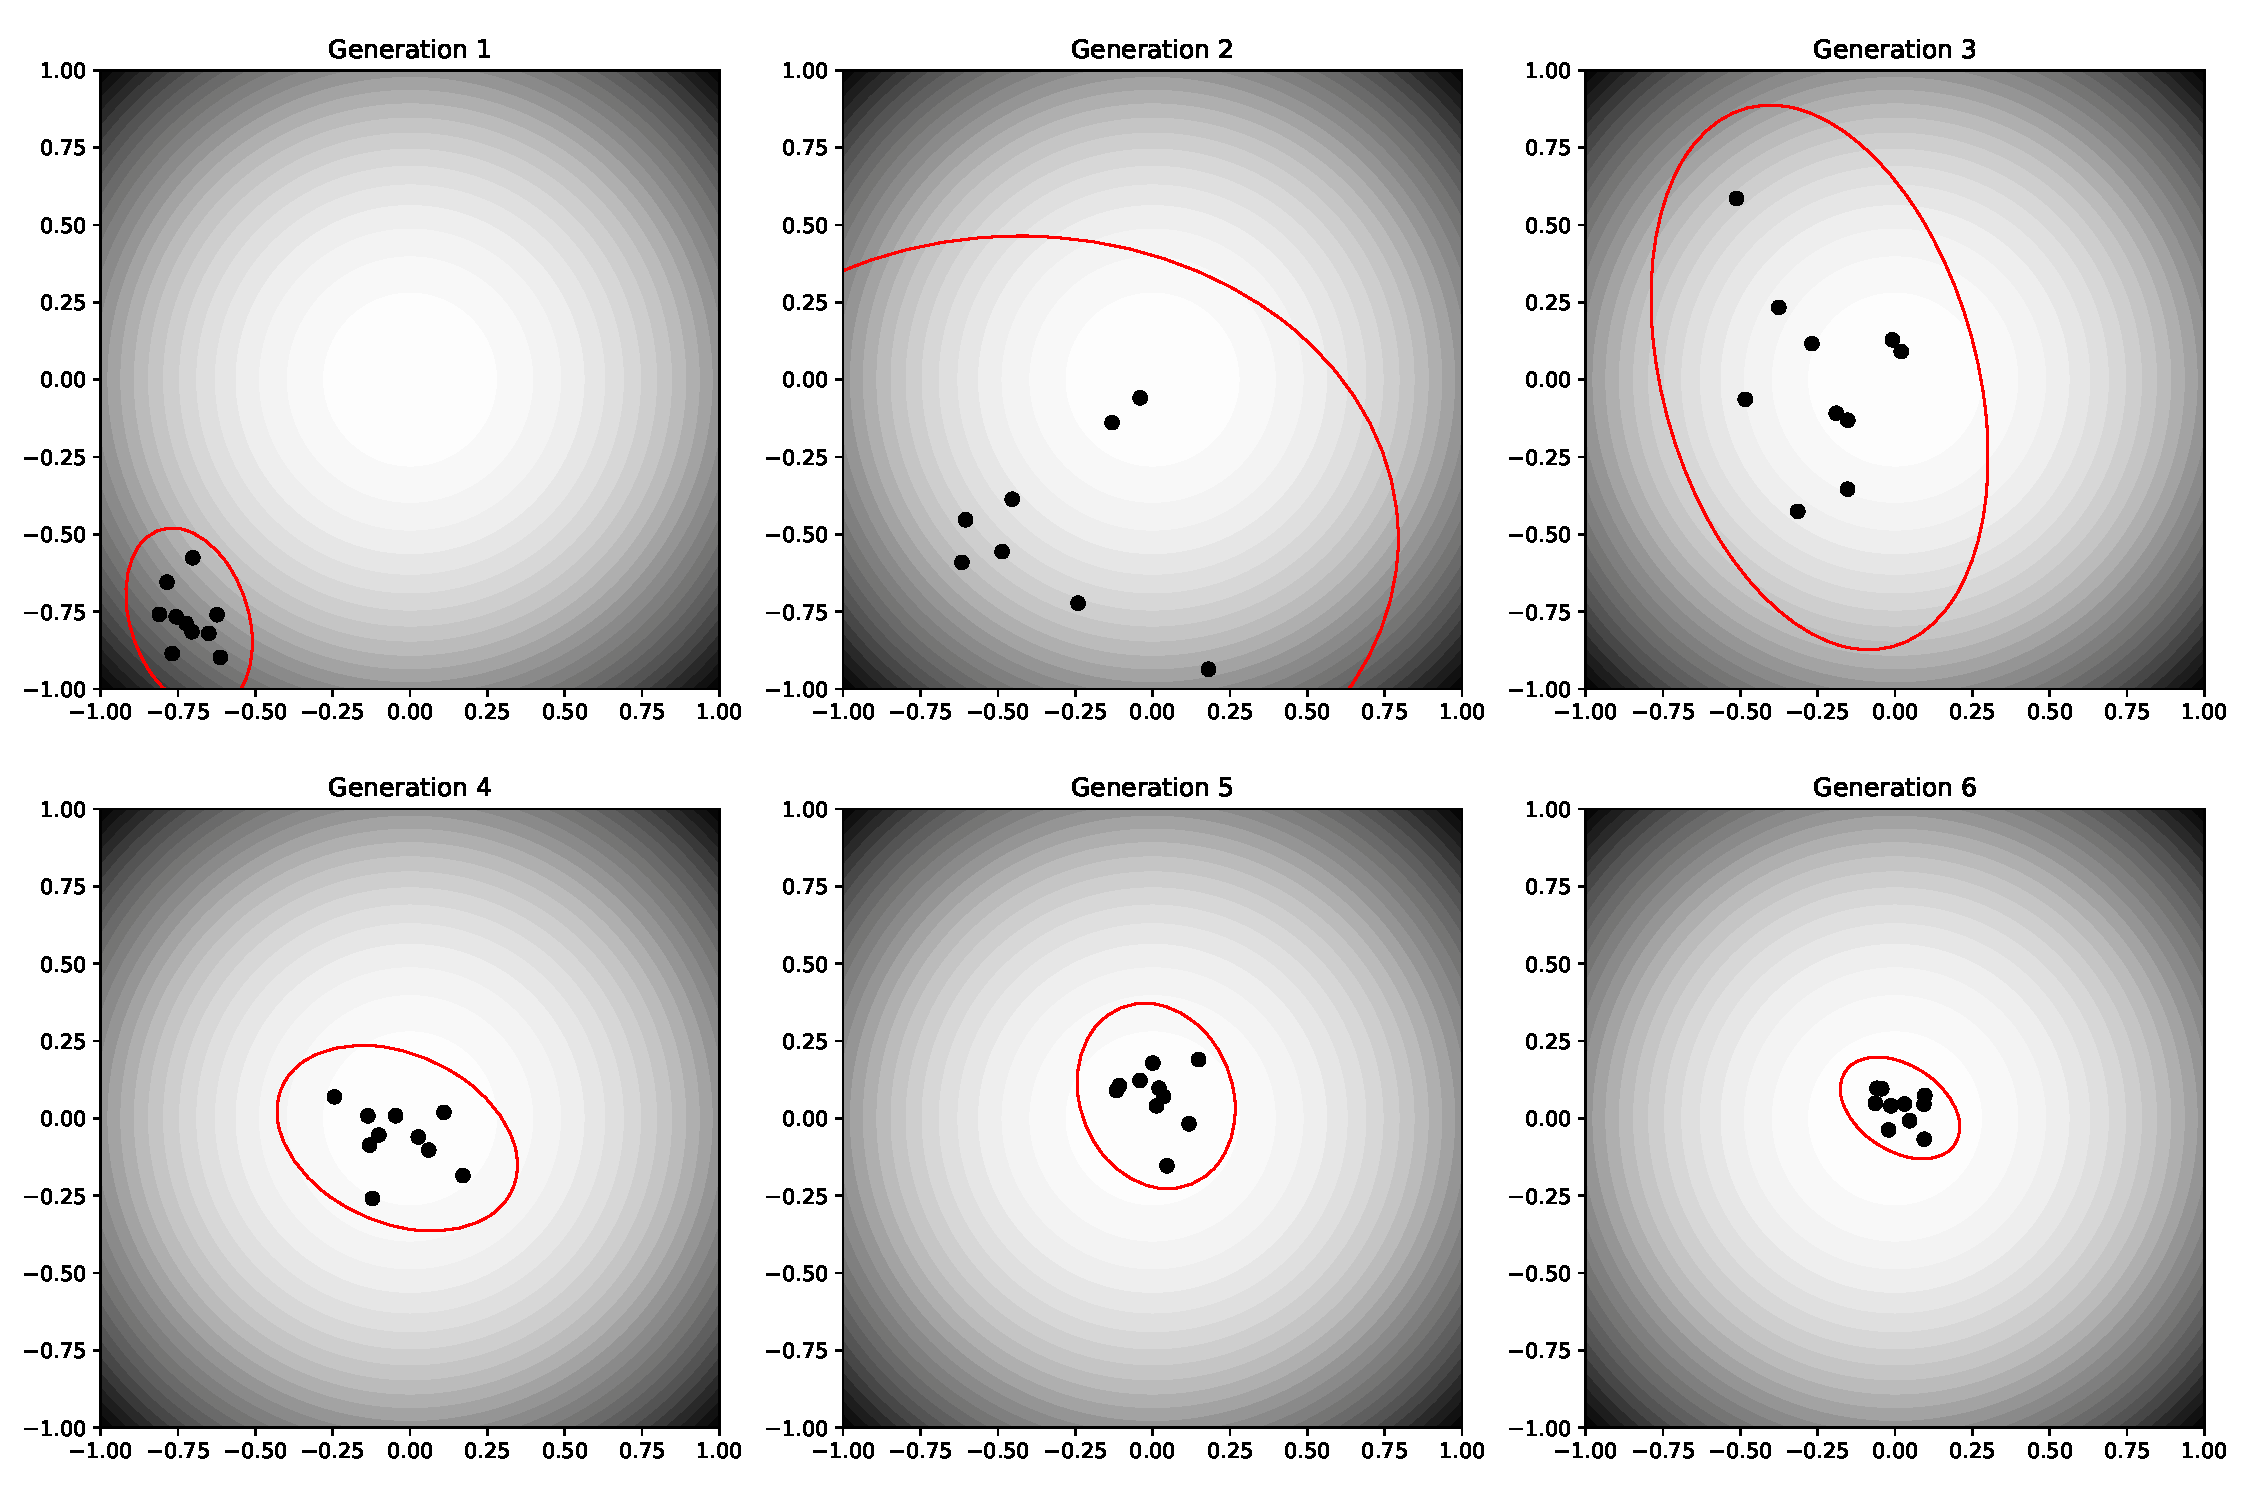
\includegraphics[width=\textwidth]{Pictures/cmaes}
    \caption{Visualization of a CMA-ES evolution process on 5 generations.
    The minimized function $f: (x,y) \in \mathds{R}^2 \to x^2 + y^2$ is depicted by lines of equal values. The mean and standard deviation of the distribution, visualized as an ellipse,
    are updated at each generation. In particular, confidence is high in the first generation, but the solution is not optimal, in future generations, a larger
    search space is used to explore the solution space, before the population concentrating around the $(0,0)$ optimum.}

    \label{fig:cmaes_visualization}
\end{figure}

\subsection{Neuroevolution of Augmenting Topologies (NEAT)}

The NEAT algorithm was introduced in \cite{neat}. It is a TWEANN (Topology and Weight Evolving Artificial Neural Network) algorithm, which evolves, simultaneously,  both
the topology and weights of neural networks. The main idea behind this algorithm is to start from a minimal topology, incrementally adding new neurons and connections to
the networks, which allows for the evolution of complex neural networks, while keeping the computational cost low and justifying each new addition to the network topology.
The following sections describe the main components of the algorithm.

\subsubsection{Genetic Encoding}

NEAT uses a direct encoding of the neural networks. The goal of the encoding strategy is to allow crossover among different network topologies.
Each genome contains two sets of genes, which specify the nodes and the connections in the network:

\begin{itemize}
    \item \textbf{Node genes} Each node gene contains an identifier and layer (input, hidden, output or bias, which is an input that is always set to $1.0$.
    \item \textbf{Connection genes} Each connection gene specifies an input node identifier, an output node identifier, a weight, whether the connection is enabled or
        disabled, and an innovation number.
\end{itemize}

An example of a genotype to phenotype mapping is shown in \Cref{fig:neat_genome}.

\begin{figure}
    \centering
    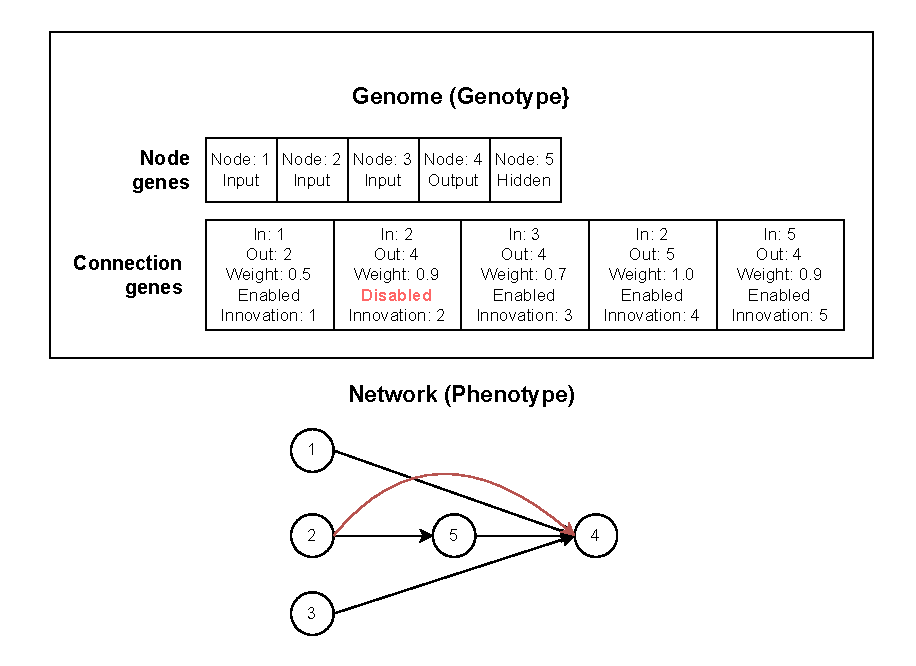
\includegraphics[width=0.9\textwidth]{Pictures/neat_encoding}
    \caption{NEAT genotype to phenotype mapping example. The disabled connection, with innovation number $2$, is not expressed in the phenotype.}
    \label{fig:neat_genome}
\end{figure}

Node identifiers are shared between the individuals in the population, the enabled flag specifies whether or not the connection is expressed in the phenotype (i.e
the network) and the innovation number is used to track the historical origin of the gene.

\subsubsection{Mutations}

NEAT uses two types of mutations: weight mutations and structural mutations. Weight mutations are used to perturb the weights of the connections in the network, while
structural mutations are used to modify the topology of the network. There are two types of structural mutations:

\begin{itemize}
    \item \textbf{Add connection} This mutation adds a new connection between two unconnected nodes in the network. The newly added connection is assigned a random weight.
    \item \textbf{Add node} This mutation adds a new node in the network, splitting an existing connection into two. The old connection is disabled and two new
        connections are added to the new node. The connection leading into the new node is assigned a weight of 1, while the connection leading out from the new node is
        assigned the weight of the old connection. This allows for the minimization of the initial effort of the mutation, as the activation of the output layer
        node remains the same and the weights of the new connections can be optimized in future generations.
\end{itemize}

Because of these two types of mutations, inserting new nodes and connection genes, genomes can only grow larger over time, resulting in the evolution of increasingly
complex networks. An example of the effect of both mutations is shown in \Cref{fig:neat_mutations}.

\begin{figure}
    \centering
    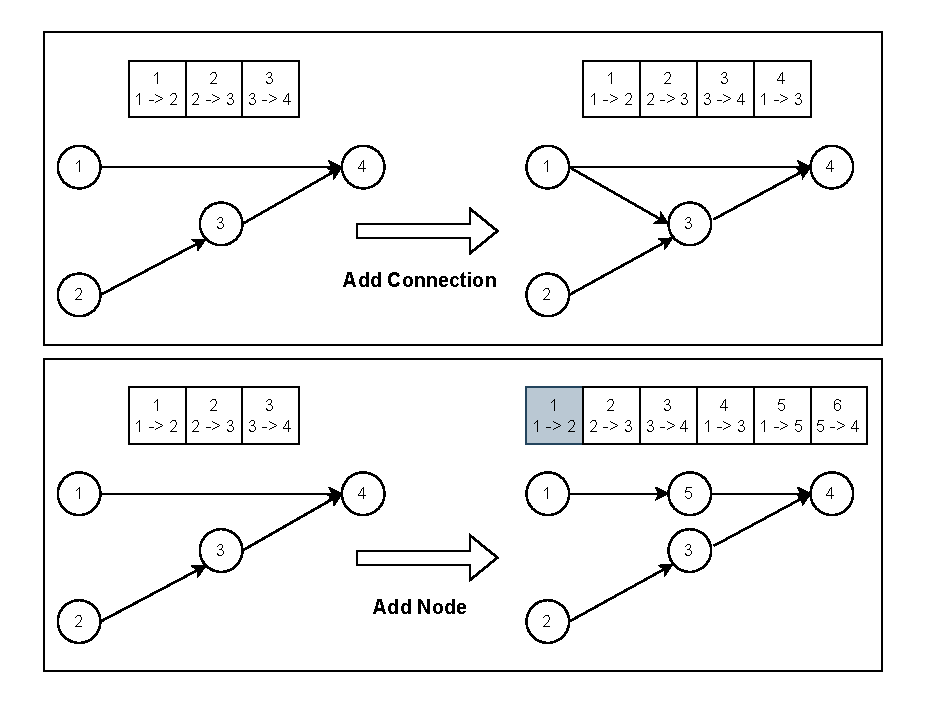
\includegraphics[width=0.9\textwidth]{Pictures/neat_mutations}
    \caption{NEAT mutations example. The add node connection mutation adds a connection between nodes $1$ and $3$.
    The add node mutation splits the connection between nodes $1$ and $4$, adding a new node $5$ and two new connections. The connection between nodes $1$ and $4$ is disabled.}
    \label{fig:neat_mutations}
\end{figure}

\subsubsection{Crossover}

One of the main challenges of evolving neural network topologies is the crossover operator, precisely because of the presence of different topologies in the population,
which makes trivial crossover operators relying on the matching of nodes and connections impossible.
NEAT addresses this issue by making use of the innovation numbers in connection genes, which allows for the tracking of the historical origin of each gene. This allows
for the matching of genes between individuals. Genes are assigned increasing innovation numbers as they appear in the population and innovation numbers are inherited.
Hence, the matching of genes is done by comparing the innovation numbers. Thus, the crossover operator consists in inheriting matching genes from one parent at random,
and adding the remaining disjoint and excess genes from the fittest parent. This strategy is particularly cost-effective as it requires no topological analysis of the networks.
An example of crossover is shown in \Cref{fig:neat_crossover}.

\begin{figure}
    \centering
    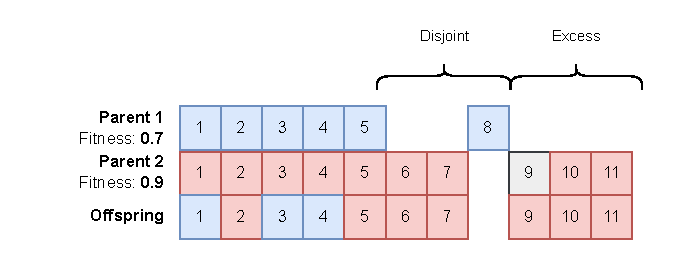
\includegraphics[width=0.9\textwidth]{Pictures/neat_crossover}
    \caption{NEAT crossover example. Matching genes are inherited from both parents at random. Disjoint and excess genes are inherited from the fittest parent. In this case, the
    disabled gene with innovation $9$ was enabled in the offspring.}
    \label{fig:neat_crossover}
\end{figure}

\subsubsection{Speciation}

An issue with the current strategy is that the population is unable to protect topological innovation, because of smaller topologies optimizing faster and the
addition of new connections usually resulting in an initial drop in fitness. To address this issue, NEAT uses speciation, which groups individuals into species based
on their genetic similarity. This strategy allows for the protection of topological innovation by having individuals compete within their specie, rather than within the
entire population. In addition, as it is the case with the crossover operator, historical matching also allows for an efficient solution to this problem.

The similarity between two individuals is computed as a weighted sum of the number of excess $E$ genes, the number of disjoint $D$ genes and the average weight difference $\bar{W}$
of matching genes:

\[
    \delta = c_1 \frac{E}{N} + c_2 \frac{D}{N} + c_3 \bar{W}.
\]

Where $c_1$, $c_2$ and $c_3$ are coefficients which control the importance of each term, and $N$ is the number of genes in the larger genome.

At each generation, individuals are sequentially assigned to a species based on their similarity with the representative of the specie, which is
a randomly selected individual from the previous generation which was part of the specie, and a similarity threshold. If no species is found, then a new species is created.

Each species is given a number of offspring in proportion to the sum of the adjusted fitness of its members. Where the adjusted fitness $f_i'$ of an individual $i$ is
given by $f_i' = f_i / n_i$, where $f_i$ is the fitness of the individual and $n_i$ is the number of individuals in the specie. This is done to prevent large species
from dominating the population. The offspring are generated using the crossover and mutation operators, on members of the species, after the selection of the fittest
individuals. At each generation, the population is replaced by the offspring. This process is repeated until a termination criterion is met.

\section{Neuroevolution benchmarks}

Neuroevolution algorithms are typically evaluated on a variety of benchmarks, which are used to test the performance of the algorithms on different problem classes.
These problems can be classified into different categories, based on the following characteristics:

\begin{itemize}
    \item \textbf{Problem type} The type of problem which is considered, such as classification, regression, control, etc.
    \item \textbf{Problem complexity} The complexity of the problem, which can be measured by the size of the state space, the number of inputs, the number of classes, etc.
    \item \textbf{The realism of the problem} The realism of the problem, which can be measured by the relevance of the problem to real-world applications, in opposition to
        toy problems which are used for theoretical studies.
\end{itemize}

\Cref{tab:neuroevolution_benchmarks} presents the benchmarks which were identified during the review. These benchmarks were found in the new algorithm proposals papers
and comparison studies. However, it is worth noting that many more benchmarks can be considered, such as any classification dataset, or the various environments implemented
in the OpenAI Gym toolkit \cite{gym}.

\begin{table}[]
\centering
\caption{Benchmarks classification}
\label{tab:neuroevolution_benchmarks}
\begin{tabular}{|c|c|c|}
\hline
\textbf{Problem}                                                                                                   & \textbf{Class} & \textbf{Variables} \\ \hline
\textbf{Unit-sphere classification} \cite{na}                                                                      & Classification & 2                  \\ \hline
\textbf{XOR} \cite{neat}                                                                                           & Classification & 2                  \\ \hline
\textbf{Double pole balancing} \cite{pole_balancing}                                                               & Control        & 6                  \\ \hline
\begin{tabular}[c]{@{}c@{}}Double pole balancing\\ (Without velocity) \cite{pole_balancing}\end{tabular}           & Control        & 3                  \\ \hline
\textbf{Proben1 Cancer1} \cite{proben}                                                                             & Classification & 9                  \\ \hline
Mountain Car \cite{mountain_car}                                                                                   & Control        & 2                  \\ \hline
Ball throwing \cite{ball_throwing}                                                                                 & Control        & 3                  \\ \hline
\end{tabular}
\end{table}

\subsection{Benchmarks selection}

The following benchmarks were selected for the implementation in the framework:

\begin{itemize}
    \item The unit-sphere classification problems
    \item The XOR problem
    \item The \textit{Proben1 Cancer1} dataset classification problem
    \item The double pole balancing problem
\end{itemize}

Once again, the choice was made to limit the number of benchmarks to four, for the same reason of allowing for an in-depth implementation and evaluation of the algorithms on each of them.
The selected benchmarks were chosen to allow for a good coverage of the different problem classes, and to allow for interesting comparisons between different algorithms or different
configurations of the same algorithm.

The double pole balancing problem was selected as a classic benchmark in the neuroevolution literature. It is the most widely used benchmark in the field, and is relevant to real-world
control problems. The unit-sphere classification problems were selected as classification toy problems, introduced in the theory paper \cite{na} and used to test the (1 + 1) NA and BNA algorithms.
Moreover, the XOR problem was selected as another classic toy classification problem, which is particularly simple, and useful for testing the ability of the algorithms to solve non-linear problems.
Lastly, the \textit{Proben1 Cancer1} dataset classification problem was selected as a more realistic classification problem, making use of a training and testing dataset, and consisting
in a higher-dimmmensional input space of $9$ features, as opposed to the $2$ features of the unit-sphere classification problems and XOR problem.

The following sections present the different benchmarks which were selected for the implementation in the framework.

\subsection{Unit hypersphere sphere classification problems}
\label{subsection:sphere_classification}

These problems, which can be thought of as a kind of \textsc{onemax} for the (1 + 1) NA algorithm, were introduced in \cite{na}.
These problems consist in the binary classification of points in the $D$-dimensional unit hypersphere.

\paragraph{Half}
The \textsc{half} problem consists of all points with non-negative $x_D$ coordinate on the unit hypersphere:

\[
    \textsc{half} = \{x \in \mathds{R}^D, \lVert x \rVert_2 = 1 \text{ and } \varphi_{D-1} \in [0, \pi]\}.
\]

\paragraph{Quarter}
The \textsc{quarter} problem consists of all points with non-negative $x_{D-1}$ and $x_D$ coordinate on the unit hypersphere:

\[
    \textsc{quarter} = \{x \in \mathds{R}^D, \lVert x \rVert_2 = 1 \text{ and } \varphi_{D-1} \in [0, \pi / 2]\}.
\]

\paragraph{TwoQuarters}
The \textsc{twoquarters} problem consists of all points with either both negative or non-negative $x_{D-1}$ and $x_D$ coordinate on the unit hypersphere:

\[
    \textsc{twoquarters} = \{x \in \mathds{R}^D, \lVert x \rVert_2 = 1 \text{ and } \varphi_{D-1} \in [0, \pi / 2] \cup [\pi, 3\pi / 2]\}.
\]

\paragraph{LocalOpt}
The \textsc{localopt} problem consists of all points with polar angle $\varphi_{D-1}$ between 0 and 60, 120 and 180, 240 and 300 degrees:

\[
    \textsc{localopt} = \{x \in \mathds{R}^D, \lVert x \rVert_2 = 1 \text{ and } \varphi_{D-1} \in [0, \pi / 3] \cup [2\pi / 3, \pi] \cup [4\pi / 3, 5\pi / 3]\}.
\]

The four problems are illustrated in \Cref{fig:sphere_classification}.

\begin{figure}
\centering
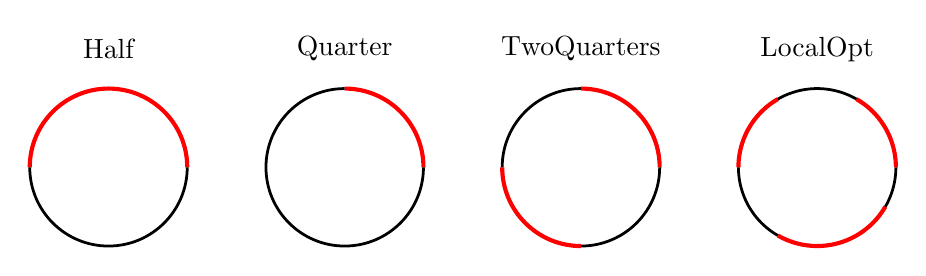
\begin{tikzpicture}
\node at (-1, 1.5) {Half};
\draw[red, line width=1.5] (0,0) arc[start angle=0, end angle=180, radius=1];
\draw[black, line width=1.0] (0,0) arc[start angle=0, end angle=-180, radius=1];

\node at (2, 1.5) {Quarter};
\draw[red, line width=1.5] (3,0) arc[start angle=0, end angle=90, radius=1];
\draw[black, line width=1.0] (3,0) arc[start angle=0, end angle=-270, radius=1];

\node at (5, 1.5) {TwoQuarters};
\draw[red, line width=1.5] (6,0) arc[start angle=0, end angle=90, radius=1];
\draw[black, line width=1.0] (6,0) arc[start angle=0, end angle=-90, radius=1];
\draw[red, line width=1.5] (4,0) arc[start angle=180, end angle=270, radius=1];
\draw[black, line width=1.0] (4,0) arc[start angle=180, end angle=90, radius=1];

\node at (8, 1.5) {LocalOpt};
\draw [red, line width=1.5, domain=0:60] plot ({8+cos(\x)}, {sin(\x)});
\draw [red, line width=1.5, domain=120:180] plot ({8+cos(\x)}, {sin(\x)});
\draw [red, line width=1.5, domain=240:330] plot ({8+cos(\x)}, {sin(\x)});
\draw [black, line width=1.0, domain=60:120] plot ({8+cos(\x)}, {sin(\x)});
\draw [black, line width=1.0, domain=180:240] plot ({8+cos(\x)}, {sin(\x)});
\draw [black, line width=1.0, domain=330:360] plot ({8+cos(\x)}, {sin(\x)});
\end{tikzpicture}
\caption{Unit hypersphere classification problems. The red area represents the positive class, while the black area represents the negative class.}
\label{fig:sphere_classification}
\end{figure}

\subsection{XOR}

This classic benchmark problem is a binary classification problem, which consists in the classification of the four points $(0, 0)$, $(0, 1)$, $(1, 0)$ and $(1, 1)$, according to the XOR function.
The points $(0, 0)$ and $(1, 1)$ are of class $0$, while the points $(0, 1)$ and $(1, 0)$ are of class $1$.
The popularity of this simple problem comes from its simplicity and non-linear nature.

\subsection{Dataset Classification Problems}

Classification using datasets is a classical use-case for neural networks.
The hypersphere toy classification problems \cite{na,} presented in \Cref{subsection:sphere_classification}, differ from this kind of task, by having
algorithms trained and tested on the same data.

Although these problems are not common use-cases for neuroevolution, because of the availability of labeled data,
they are particularly interesting for this study, by allowing to show how neuroevolution can be applied to these common tasks, testing
the algorithms on larger state spaces, and potentially observing whether common behaviors which occur when training ANNs using gradient-based methods,
such as over-fitting or under-fitting, also apply to neuroevolution \cite{overfitting}.

The \textit{Proben1} benchmarks, presented in \cite{proben}, introduce various standard benchmark datasets, including the \textit{Cancer 1} dataset, which
contains $699$ entries, consisting in cell descriptors gathered by microscopic analysis for tumors being benign or malignant.
Each dataset entry contains $9$ input features, and a binary output,

\subsection{Pole Balancing}

The pole balancing problem, as described in \cite{pole_balancing}, is a classical benchmark in control theory, reinforcement learning and neuroevolution literature.
It consists in controlling a cart, with one degree of freedom, moving along a one-dimensional track, by applying a horizontal force to it in order to balance a pole attached to it using a hinge.
Some of the reasons for the popularity of this benchmark problem are its simplicity, its relevance to real-world control problems and its unstable and non-linear dynamics.

% TODO pole balancing figure

The difficulty of the problem can be adjusted by changing the number of poles. Indeed, if the poles have different lengths, they will react differently to the forces applied to the cart
and it would be able to balance them.
As the single pole variant has become too easy for current techniques, we consider the widely used case of double pole balancing, where two poles are attached to the cart.

The state of the system is described by the cart position $x$, the cart velocity $\dot{x}$, the pole angles $\theta_1$ and $\theta_2$ and the angular velocities $\dot{\theta}_1$ and $\dot{\theta}_2$.
A visualisation of the problem is shown in \Cref{fig:pole_balancing}.
This task is Markovian, as the state contains all the information needed to determine the future evolution of the system.
A more challenging variant of the problem consists in removing the velocity informations from the state, which requires the use of recurrent connections, which were not considered
in this project.

\begin{figure}
    \centering
    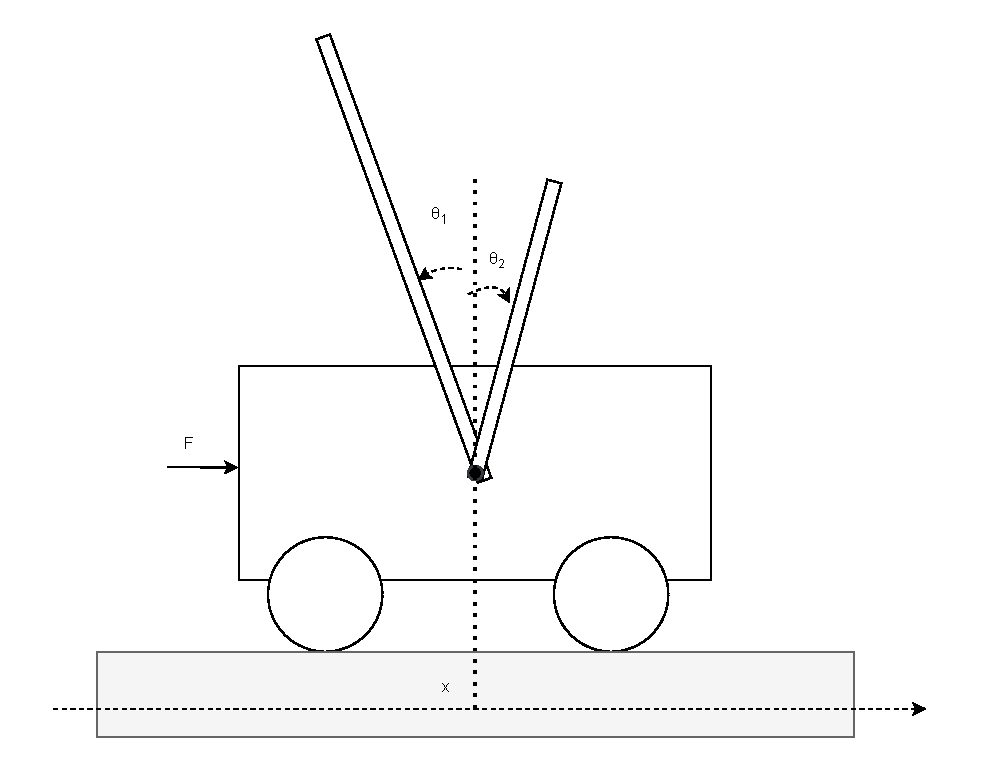
\includegraphics[width=0.8\textwidth]{Pictures/cart_pole}
    \caption{Double pole balancing problem. The cart is controlled by applying a force of magnitude $F$ to it, in order to balance the two poles attached to it.}
    \label{fig:pole_balancing}
\end{figure}

The dynamics of the system are described by the following equations:

\[
    \begin{aligned}
        \ddot{x} &= \frac{F - \mu_c \text{sgn}(\dot{x}) + \sum_{i = 1}^N \tilde{F_i}}{M + \sum_{i = 1}^N \tilde{m_i}} \\
        \forall i \in \{1, N\}, \ddot{\theta_i} &= - \frac{3}{4 l_i} (\ddot{x} \cos \theta_i + g \sin \theta_i + \frac{\mu_{pi} \dot{\theta_i}}{m_i l_i})\\
        \forall i \in \{1, N\}, \tilde{F_i} &= m_i l_i \dot{\theta_i}^2 \sin \theta_i + \frac{3}{4} m_i \cos \theta_i (\frac{\mu_{pi} \dot{\theta_i}}{m_i l_i} + g \sin \theta_i) \\
        \tilde{m_i} &= \m_i (1 - \frac{3}{4} \cos^2 \theta_i). \\
    \end{aligned}
\]

Where:

\begin{itemize}
    \item $F$ is the magnitude of the force applied to the cart
    \item $\mu_c$ is the cart friction coefficient
    \item $M$ is the cart mass
    \item $N$ is the number of poles
    \item $l_i$ is the length of the $i$-th pole
    \item $\mu_{pi}$ is the pole friction coefficient
    \item $m_i$ is the mass of the $i$-th pole
    \item $g$ is the gravity constant
\end{itemize}

The equations for motion are integrated using the Euler method \cite{euler}. For a time step $\Delta t$:

\[
    \begin{aligned}
        x_{t+1} &= x_t + \dot{x}_t \Delta t \\
        \dot{x}_{t+1} &= \dot{x}_t + \ddot{x}_t \Delta t \\
        \theta_{i, t+1} &= \theta_{i, t} + \dot{\theta}_{i, t} \Delta t \\
        \dot{\theta}_{i, t+1} &= \dot{\theta}_{i, t} + \ddot{\theta}_{i, t} \Delta t. \\
    \end{aligned}
\]

The fitness function is defined as the sum of the time steps during which the poles are balanced and the cart is within the allowed bounds, over a maximum of $1000$ time steps.
A pole is considered balanced if its angle is within $30$ degrees of the vertical position.
The evaluated algorithms outputs are mapped to the magnitude of the force $F \in [-10, 10]$N (Newtons) to be applied to the cart at each time step.

\section{Related Work}

Various works evaluate the performance of neuroevolution algorithms on different benchmarks, and compare them to other algorithms.
First of all, all of the selected algorithms were evaluated on a selection of benchmarks in thei original papers.
Both the (1 + 1) NA and BNA algorithms were evaluated on the unit-sphere classification problems \cite{na, bna}, and NEAT was evaluated on the XOR and pole balancing problems \cite{neat}.
Moreover, BNA is compared to (1 + 1) NA on the unit-sphere classification problems in \cite{bna}, which was also compared to the use of the CMA-ES algorithm on the descibed ANN architecture in
\cite{na}. However, both studies did not compare these algorithms to other neuroevolution algorithms, and as these theory algorithms are not used in practice, they are not the subject of
coparison to other neuroevolution algorithms in other studies. This is a research gap which this study aims to address.
Regarding NEAT and CMA-ES, both algorithms were re-evaluated and compared on the double pole balancing problem in \cite{neuroevolution_es_rl}, and, among other problems, in \cite{robust}.
